Loading initial resources:

\begin{Shaded}
\begin{Highlighting}[]
\KeywordTok{library}\NormalTok{(tidyverse)}
\KeywordTok{library}\NormalTok{(magrittr)}
\KeywordTok{library}\NormalTok{(geneplast)}
\KeywordTok{library}\NormalTok{(ape)}
\KeywordTok{library}\NormalTok{(XML)}
\KeywordTok{library}\NormalTok{(rentrez)}
\KeywordTok{library}\NormalTok{(neurotransmissionevolution)}

\KeywordTok{data}\NormalTok{(}
\NormalTok{  cogs,}
\NormalTok{  gene_cogs,}
\NormalTok{  string_eukaryotes,}
  \DataTypeTok{package =} \StringTok{"neurotransmissionevolution"}
\NormalTok{)}

\NormalTok{phyloTree <-}\StringTok{ }\KeywordTok{read.tree}\NormalTok{(}\StringTok{"../data/hybrid_tree_modified.nwk"}\NormalTok{) }\OperatorTok\StringTok{ }\KeywordTok{rotatePhyloTree}\NormalTok{(}\StringTok{"9606"}\NormalTok{)}
\end{Highlighting}
\end{Shaded}

We perform some minor data formatting before feeding it to geneplast

\begin{Shaded}
\begin{Highlighting}[]
\CommentTok{# Formating cogdata column names for geneplast}
\NormalTok{cogs }\OperatorTok\StringTok{ }\KeywordTok{rename}\NormalTok{(}\DataTypeTok{protein_id =}\NormalTok{ string_id, }\DataTypeTok{ssp_id =}\NormalTok{ taxid) }\OperatorTok\StringTok{ }\KeywordTok{select}\NormalTok{(protein_id, ssp_id, cog_id)}

\CommentTok{# Adding species names to taxid tree}
\NormalTok{phyloTree }\OperatorTok\StringTok{ }\KeywordTok{list_modify}\NormalTok{(}
  \DataTypeTok{tip.alias =}\NormalTok{ string_eukaryotes }\OperatorTok\StringTok{ }\NormalTok{string_name[}\KeywordTok{match}\NormalTok{(phyloTree[[}\StringTok{"tip.label"}\NormalTok{]], taxid)]}
\NormalTok{)}
\end{Highlighting}
\end{Shaded}

\hypertarget{geneplast}{%
\subsubsection{Geneplast}\label{geneplast}}

Geneplast's \texttt{groot.preprocess} function structures an
\texttt{ogr} object on which \texttt{groot} will perform the rooting. We
then retrieve the numeric root (\texttt{groot.get("results")}) for the
\texttt{cogs\_of\_interest}, that is, orthologous groups pertaining to
neurotransmission genes.

\begin{Shaded}
\begin{Highlighting}[]
\NormalTok{cogs_of_interest <-}\StringTok{ }\NormalTok{gene_cogs }\OperatorTok\StringTok{ }\KeywordTok{pull}\NormalTok{(cog_id) }\OperatorTok\StringTok{ }\NormalTok{unique}

\NormalTok{ogr <-}\StringTok{ }\KeywordTok{groot.preprocess}\NormalTok{(}
  \DataTypeTok{cogdata   =}\NormalTok{ cogs,}
  \DataTypeTok{phyloTree =}\NormalTok{ phyloTree,}
  \DataTypeTok{spid      =} \StringTok{"9606"}\NormalTok{,}
  \DataTypeTok{cogids    =}\NormalTok{ cogs_of_interest}
\NormalTok{)}

\NormalTok{roots <-}\StringTok{ }\KeywordTok{groot}\NormalTok{(ogr, }\DataTypeTok{nPermutations =} \DecValTok{1}\NormalTok{) }\OperatorTok
\StringTok{  }\KeywordTok{groot.get}\NormalTok{(}\StringTok{"results"}\NormalTok{) }\OperatorTok
\StringTok{  }\KeywordTok{rownames_to_column}\NormalTok{(}\StringTok{"cog_id"}\NormalTok{) }\OperatorTok
\StringTok{  }\KeywordTok{select}\NormalTok{(cog_id, }\DataTypeTok{root =}\NormalTok{ Root) }\OperatorTok
\StringTok{  }\KeywordTok{write_tsv}\NormalTok{(}\StringTok{"geneplast_roots.tsv"}\NormalTok{)}
\end{Highlighting}
\end{Shaded}

\hypertarget{clade-names}{%
\subsubsection{Clade names}\label{clade-names}}

Each root branches to a clade that diverged from humans some time in the
past. It is nice to have these clades taxonomically named to ease our
interpretation. Unlike NCBI Taxonomy, TimeTree's internal nodes are not
named. Therefore, we query the NCBI Taxonomy API to try to find most
clade names automatically. It is important to note that we are using a
hybrid tree primarily built from TimeTree data. This means NCBI Taxonomy
naming will not perfectly match clades in our tree. For instance, root
\#36 branches to a clade containing 38 species from the SAR supergroup,
but also 1 species from the Haptista rank, namely \emph{Emiliania
huxleyi}. The Haptista group is a sister clade to SAR, so it might be
the case that \emph{Emiliania huxleyi} is actually correctly placed
together with SAR species by TimeTree, given their evolutionary
proximity. Resolving these naming conflicts is not trivial and falls out
of our scope.

\begin{Shaded}
\begin{Highlighting}[]
\NormalTok{lineages <-}\StringTok{ }\KeywordTok{entrez_fetch}\NormalTok{(}
  \DataTypeTok{db      =} \StringTok{"taxonomy"}\NormalTok{,}
  \DataTypeTok{id      =}\NormalTok{ string_eukaryotes[[}\StringTok{"new_taxid"}\NormalTok{]],}
  \DataTypeTok{rettype =} \StringTok{"xml"}\NormalTok{,}
  \DataTypeTok{retmode =} \StringTok{"xml"}\NormalTok{,}
  \DataTypeTok{parsed  =} \OtherTok{TRUE}
\NormalTok{)}

\NormalTok{string_eukaryotes }\OperatorTok\StringTok{ }\KeywordTok{mutate}\NormalTok{(}
  \DataTypeTok{root        =}\NormalTok{ ogr}\OperatorTok{@}\NormalTok{tree}\OperatorTok{$}\NormalTok{tip.group[taxid],}
  \DataTypeTok{lineage_txt =} \KeywordTok{xpathSApply}\NormalTok{(lineages, }\StringTok{"//Lineage"}\NormalTok{, XML}\OperatorTok{::}\NormalTok{xmlValue)}
\NormalTok{)}

\KeywordTok{write}\NormalTok{(string_eukaryotes[[}\StringTok{"lineage_txt"}\NormalTok{]], }\StringTok{"temp/species_lineages.txt"}\NormalTok{)}
  
\CommentTok{# collapse_names(c("a","b","a")) == "a (2); b (1)"}
\NormalTok{collapse_names <-}\StringTok{ }\ControlFlowTok{function}\NormalTok{(clade_names) \{}
  \KeywordTok{table}\NormalTok{(clade_names) }\OperatorTok\StringTok{ }\KeywordTok{sort}\NormalTok{(}\OtherTok{TRUE}\NormalTok{) }\OperatorTok\StringTok{ }\KeywordTok{paste0}\NormalTok{(}\KeywordTok{names}\NormalTok{(.), }\StringTok{" ("}\NormalTok{, .,}\StringTok{")"}\NormalTok{, }\DataTypeTok{collapse =} \StringTok{"; "}\NormalTok{)}
\NormalTok{\}}

\NormalTok{root_names <-}\StringTok{ }\NormalTok{string_eukaryotes }\OperatorTok
\StringTok{  }\CommentTok{# Long format lineages}
\StringTok{  }\KeywordTok{mutate}\NormalTok{(}
     \DataTypeTok{lineage_split =} \KeywordTok{strsplit}\NormalTok{(lineage_txt, }\StringTok{"; "}\NormalTok{)}
\NormalTok{  ) }\OperatorTok
\StringTok{  }\KeywordTok{unnest_longer}\NormalTok{(}
     \DataTypeTok{col             =}\NormalTok{ lineage_split}
\NormalTok{    ,}\DataTypeTok{values_to       =} \StringTok{"clade_name"}
\NormalTok{    ,}\DataTypeTok{indices_to      =} \StringTok{"clade_depth"}
\NormalTok{  ) }\OperatorTok
\StringTok{  }\CommentTok{# Collapsing lineages at clade ranks}
\StringTok{  }\KeywordTok{group_by}\NormalTok{(root, clade_depth) }\OperatorTok
\StringTok{  }\KeywordTok{summarise}\NormalTok{(}
     \DataTypeTok{diverging_rank =} \KeywordTok{n_distinct}\NormalTok{(clade_name) }\OperatorTok{>}\StringTok{ }\DecValTok{1}
\NormalTok{    ,}\DataTypeTok{clade_name     =} \KeywordTok{ifelse}\NormalTok{(diverging_rank, }\KeywordTok{collapse_names}\NormalTok{(clade_name), clade_name)}
\NormalTok{  ) }\OperatorTok
\StringTok{  }\CommentTok{# Removing subsequent divergences}
\StringTok{  }\KeywordTok{filter}\NormalTok{(}\KeywordTok{cumsum}\NormalTok{(diverging_rank) }\OperatorTok{<=}\StringTok{ }\DecValTok{1}\NormalTok{) }\OperatorTok
\StringTok{  }\CommentTok{# Removing irrelevant ranks}
\StringTok{  }\KeywordTok{group_by}\NormalTok{(clade_depth) }\OperatorTok
\StringTok{  }\KeywordTok{arrange}\NormalTok{(root) }\OperatorTok
\StringTok{  }\KeywordTok{filter}\NormalTok{(}\OperatorTok{!}\NormalTok{(}\KeywordTok{duplicated}\NormalTok{(clade_name) }\OperatorTok{|}\StringTok{ }\KeywordTok{duplicated}\NormalTok{(clade_name, }\DataTypeTok{fromLast =} \OtherTok{TRUE}\NormalTok{)) }\OperatorTok{|}\StringTok{ }\NormalTok{diverging_rank) }\OperatorTok
\StringTok{  }\CommentTok{# Choosing name}
\StringTok{  }\KeywordTok{group_by}\NormalTok{(root) }\OperatorTok
\StringTok{  }\KeywordTok{summarise}\NormalTok{(}\DataTypeTok{clade_name =} \KeywordTok{first}\NormalTok{(clade_name, }\DataTypeTok{order_by =}\NormalTok{ clade_depth)) }\OperatorTok
\StringTok{  }\KeywordTok{write_tsv}\NormalTok{(}\StringTok{"temp/temp_geneplast_clade_names.tsv"}\NormalTok{)}
\end{Highlighting}
\end{Shaded}

Some automatically named clades are resolved by hand. The following
table shows clade names before and after manual checking:

\begin{Shaded}
\begin{Highlighting}[]
\CommentTok{# Loading manually resolved names, based on temp/temp_geneplast_clade_names.tsv}
\NormalTok{lca_names <-}\StringTok{ }\KeywordTok{read_tsv}\NormalTok{(}\StringTok{"geneplast_clade_names.tsv"}\NormalTok{)}

\NormalTok{root_names }\OperatorTok
\StringTok{  }\KeywordTok{rename}\NormalTok{(}\StringTok{"automatic_name"}\NormalTok{ =}\StringTok{ }\NormalTok{clade_name) }\OperatorTok
\StringTok{  }\KeywordTok{inner_join}\NormalTok{(lca_names) }\OperatorTok
\StringTok{  }\KeywordTok{rename}\NormalTok{(}\StringTok{"corrected_name"}\NormalTok{ =}\StringTok{ }\NormalTok{clade_name) }\OperatorTok
\StringTok{  }\NormalTok{knitr}\OperatorTok{::}\KeywordTok{kable}\NormalTok{(}\DataTypeTok{caption =} \StringTok{"Clade names before and after manual checking."}\NormalTok{, }\DataTypeTok{booktabs =} \OtherTok{TRUE}\NormalTok{, }\DataTypeTok{linesep =} \StringTok{""}\NormalTok{) }\OperatorTok
\StringTok{  }\NormalTok{kableExtra}\OperatorTok{::}\KeywordTok{kable_styling}\NormalTok{(}\DataTypeTok{position =} \StringTok{"left"}\NormalTok{, }\DataTypeTok{latex_options =} \KeywordTok{c}\NormalTok{(}\StringTok{"striped"}\NormalTok{, }\StringTok{"HOLD_position"}\NormalTok{))}
\end{Highlighting}
\end{Shaded}

\begin{table}[H]

\caption{\label{tab:unnamed-chunk-6}Clade names before and after manual checking.}
\begin{tabular}[t]{rll}
\toprule
root & automatic\_name & corrected\_name\\
\midrule
\rowcolor{gray!6}  1 & Homo & Homo\\
2 & Pan & Pan\\
\rowcolor{gray!6}  3 & Gorilla & Gorilla\\
4 & Ponginae & Ponginae\\
\rowcolor{gray!6}  5 & Hylobatidae & Hylobatidae\\
6 & Cercopithecoidea & Cercopithecoidea\\
\rowcolor{gray!6}  7 & Platyrrhini & Platyrrhini\\
8 & Tarsiiformes & Tarsiiformes\\
\rowcolor{gray!6}  9 & Strepsirrhini & Strepsirrhini\\
10 & Dermoptera & Dermoptera\\
\rowcolor{gray!6}  11 & Scandentia & Scandentia\\
12 & Glires & Glires\\
\rowcolor{gray!6}  13 & Laurasiatheria & Laurasiatheria\\
14 & Afrotheria (6); Xenarthra (1) & Afrotheria\\
\rowcolor{gray!6}  15 & Metatheria & Metatheria\\
16 & Prototheria & Prototheria\\
\rowcolor{gray!6}  17 & Sauropsida & Sauropsida\\
18 & Amphibia & Amphibia\\
\rowcolor{gray!6}  19 & Coelacanthimorpha & Coelacanthimorpha\\
20 & Actinopterygii & Actinopterygii\\
\rowcolor{gray!6}  21 & Tunicata & Tunicata\\
22 & Cephalochordata & Cephalochordata\\
\rowcolor{gray!6}  23 & Echinodermata (1); Hemichordata (1) & Ambulacraria\\
24 & Ecdysozoa (43); Spiralia (2) & Ecdysozoa\\
\rowcolor{gray!6}  25 & Spiralia & Spiralia\\
26 & Cnidaria & Cnidaria\\
\rowcolor{gray!6}  27 & Placozoa & Placozoa\\
28 & Porifera & Porifera\\
\rowcolor{gray!6}  29 & Ctenophora & Ctenophora\\
30 & Opisthokonta (5); Apusozoa (1); Cryptophyceae (1) & Choanoflagellata\\
\rowcolor{gray!6}  31 & Fungi & Fungi\\
32 & Amoebozoa & Amoebozoa\\
\rowcolor{gray!6}  33 & Viridiplantae & Viridiplantae\\
34 & Discoba (6); Metamonada (1); Sar (1) & Discoba\\
\rowcolor{gray!6}  35 & Rhodophyta & Rhodophyta\\
36 & Sar (38); Haptista (1) & SAR\\
\rowcolor{gray!6}  37 & Metamonada & Metamonada\\
\bottomrule
\end{tabular}
\end{table}

\hypertarget{phyletic-patterns}{%
\subsubsection{Phyletic patterns}\label{phyletic-patterns}}

Visualizing the presence/absence matrix according to inferred roots and
species' clades

\begin{Shaded}
\begin{Highlighting}[]
\NormalTok{lca_names }\OperatorTok\StringTok{ }\KeywordTok{rename}\NormalTok{(}\StringTok{"lca"}\NormalTok{ =}\StringTok{ }\NormalTok{root)}

\NormalTok{lca_spp <-}\StringTok{ }\NormalTok{ogr}\OperatorTok{@}\NormalTok{spbranches }\OperatorTok
\StringTok{  }\KeywordTok{rename}\NormalTok{(}\StringTok{"taxid"}\NormalTok{ =}\StringTok{ }\NormalTok{ssp_id, }\StringTok{"species"}\NormalTok{ =}\StringTok{ }\NormalTok{ssp_name, }\StringTok{"lca"}\NormalTok{ =}\StringTok{ `}\DataTypeTok{9606}\StringTok{`}\NormalTok{) }\OperatorTok
\StringTok{  }\KeywordTok{mutate}\NormalTok{(}\DataTypeTok{taxid_order =} \KeywordTok{row_number}\NormalTok{())}
  
\CommentTok{# Saving for use in abundance computation}
\NormalTok{lca_spp }\OperatorTok\StringTok{ }\KeywordTok{select}\NormalTok{(lca, taxid, taxid_order) }\OperatorTok\StringTok{ }\KeywordTok{write_tsv}\NormalTok{(}\StringTok{"geneplast_clade_taxids.tsv"}\NormalTok{)}

\NormalTok{cog_pam <-}\StringTok{ }\NormalTok{ogr}\OperatorTok{@}\NormalTok{orthoct[,}\OperatorTok{-}\DecValTok{1}\NormalTok{]}

\NormalTok{long_pam <-}\StringTok{ }\NormalTok{cog_pam }\OperatorTok
\StringTok{  }\KeywordTok{rownames_to_column}\NormalTok{(}\StringTok{"taxid"}\NormalTok{) }\OperatorTok
\StringTok{  }\KeywordTok{pivot_longer}\NormalTok{(}\OperatorTok{-}\NormalTok{taxid, }\DataTypeTok{names_to =} \StringTok{"cog_id"}\NormalTok{) }\OperatorTok
\StringTok{  }\KeywordTok{left_join}\NormalTok{(lca_spp) }\OperatorTok
\StringTok{  }\KeywordTok{left_join}\NormalTok{(lca_names) }\OperatorTok
\StringTok{  }\KeywordTok{left_join}\NormalTok{(roots) }\OperatorTok
\StringTok{  }\KeywordTok{mutate}\NormalTok{(}
    \DataTypeTok{cog_id       =} \KeywordTok{fct_reorder}\NormalTok{(cog_id, root),}
    \DataTypeTok{species      =} \KeywordTok{fct_reorder}\NormalTok{(species, }\KeywordTok{desc}\NormalTok{(taxid_order)),}
    \DataTypeTok{clade_name   =} \KeywordTok{fct_reorder}\NormalTok{(clade_name, lca),}
    \DataTypeTok{root         =} \KeywordTok{as_factor}\NormalTok{(root),}
    \DataTypeTok{clade_stripe =} \KeywordTok{as.numeric}\NormalTok{(}\KeywordTok{as_factor}\NormalTok{(lca)) }\OperatorTok\StringTok{ }\DecValTok{2} \OperatorTok{==}\StringTok{ }\DecValTok{0}
\NormalTok{  ) }\OperatorTok
\StringTok{  }\CommentTok{# Stripe every other species}
\StringTok{  }\KeywordTok{group_by}\NormalTok{(cog_id) }\OperatorTok
\StringTok{  }\KeywordTok{mutate}\NormalTok{(}\DataTypeTok{spp_stripe =} \KeywordTok{as.numeric}\NormalTok{(species) }\OperatorTok\StringTok{ }\DecValTok{2} \OperatorTok{==}\StringTok{ }\DecValTok{0}\NormalTok{) }\OperatorTok
\StringTok{  }\CommentTok{# Removing empty tiles}
\StringTok{  }\KeywordTok{filter}\NormalTok{(value }\OperatorTok{==}\StringTok{ }\DecValTok{1}\NormalTok{) }\OperatorTok
\StringTok{  }\CommentTok{# Stripe every other cog}
\StringTok{  }\KeywordTok{group_by}\NormalTok{(taxid) }\OperatorTok
\StringTok{  }\KeywordTok{mutate}\NormalTok{(}\DataTypeTok{cog_stripe =} \KeywordTok{as.numeric}\NormalTok{(cog_id) }\OperatorTok\StringTok{ }\DecValTok{2} \OperatorTok{==}\StringTok{ }\DecValTok{0}\NormalTok{)}

\KeywordTok{ggplot}\NormalTok{(long_pam, }\KeywordTok{aes}\NormalTok{(}\DataTypeTok{x =}\NormalTok{ cog_id, }\DataTypeTok{y =}\NormalTok{ species)) }\OperatorTok{+}
\StringTok{  }\KeywordTok{geom_tile}\NormalTok{(}\KeywordTok{aes}\NormalTok{(}\DataTypeTok{fill =}\NormalTok{ clade_stripe }\OperatorTok{+}\StringTok{ }\FloatTok{0.3} \OperatorTok{*}\StringTok{ }\KeywordTok{xor}\NormalTok{(spp_stripe, cog_stripe))) }\OperatorTok{+}
\StringTok{  }\KeywordTok{scale_fill_gradient}\NormalTok{(}\DataTypeTok{low =} \StringTok{"#37474F"}\NormalTok{, }\DataTypeTok{high =} \StringTok{"#263238"}\NormalTok{) }\OperatorTok{+}
\StringTok{  }\KeywordTok{facet_grid}\NormalTok{(clade_name }\OperatorTok{~}\StringTok{ }\KeywordTok{fct_rev}\NormalTok{(root), }\DataTypeTok{scales =} \StringTok{"free"}\NormalTok{, }\DataTypeTok{space=}\StringTok{'free'}\NormalTok{) }\OperatorTok{+}
\StringTok{  }\KeywordTok{theme}\NormalTok{(}
    \DataTypeTok{text               =} \KeywordTok{element_text}\NormalTok{(}\DataTypeTok{size =} \DecValTok{2}\NormalTok{),}
    \DataTypeTok{panel.spacing      =} \KeywordTok{unit}\NormalTok{(}\DecValTok{1}\NormalTok{, }\StringTok{"pt"}\NormalTok{),}
    \DataTypeTok{panel.grid.major.x =} \KeywordTok{element_blank}\NormalTok{(),}
    \DataTypeTok{strip.background   =} \KeywordTok{element_rect}\NormalTok{(}\DataTypeTok{colour =} \StringTok{"#FFFFFF"}\NormalTok{),}
    \DataTypeTok{strip.text.x       =} \KeywordTok{element_text}\NormalTok{(}\DataTypeTok{size =} \DecValTok{6}\NormalTok{, }\DataTypeTok{angle =} \DecValTok{90}\NormalTok{),}
    \DataTypeTok{strip.text.y       =} \KeywordTok{element_text}\NormalTok{(}\DataTypeTok{size =} \DecValTok{3}\NormalTok{, }\DataTypeTok{angle =} \DecValTok{0}\NormalTok{, }\DataTypeTok{hjust =} \DecValTok{0}\NormalTok{, }\DataTypeTok{lineheight =} \DecValTok{3}\NormalTok{),}
    \DataTypeTok{axis.text.x        =} \KeywordTok{element_text}\NormalTok{(}\DataTypeTok{size =} \DecValTok{6}\NormalTok{, }\DataTypeTok{angle =} \DecValTok{-45}\NormalTok{, }\DataTypeTok{vjust =} \DecValTok{0}\NormalTok{, }\DataTypeTok{hjust =} \DecValTok{0}\NormalTok{),}
    \DataTypeTok{legend.position    =} \StringTok{"none"}
\NormalTok{  )}
\end{Highlighting}
\end{Shaded}

\begin{figure}

{\centering 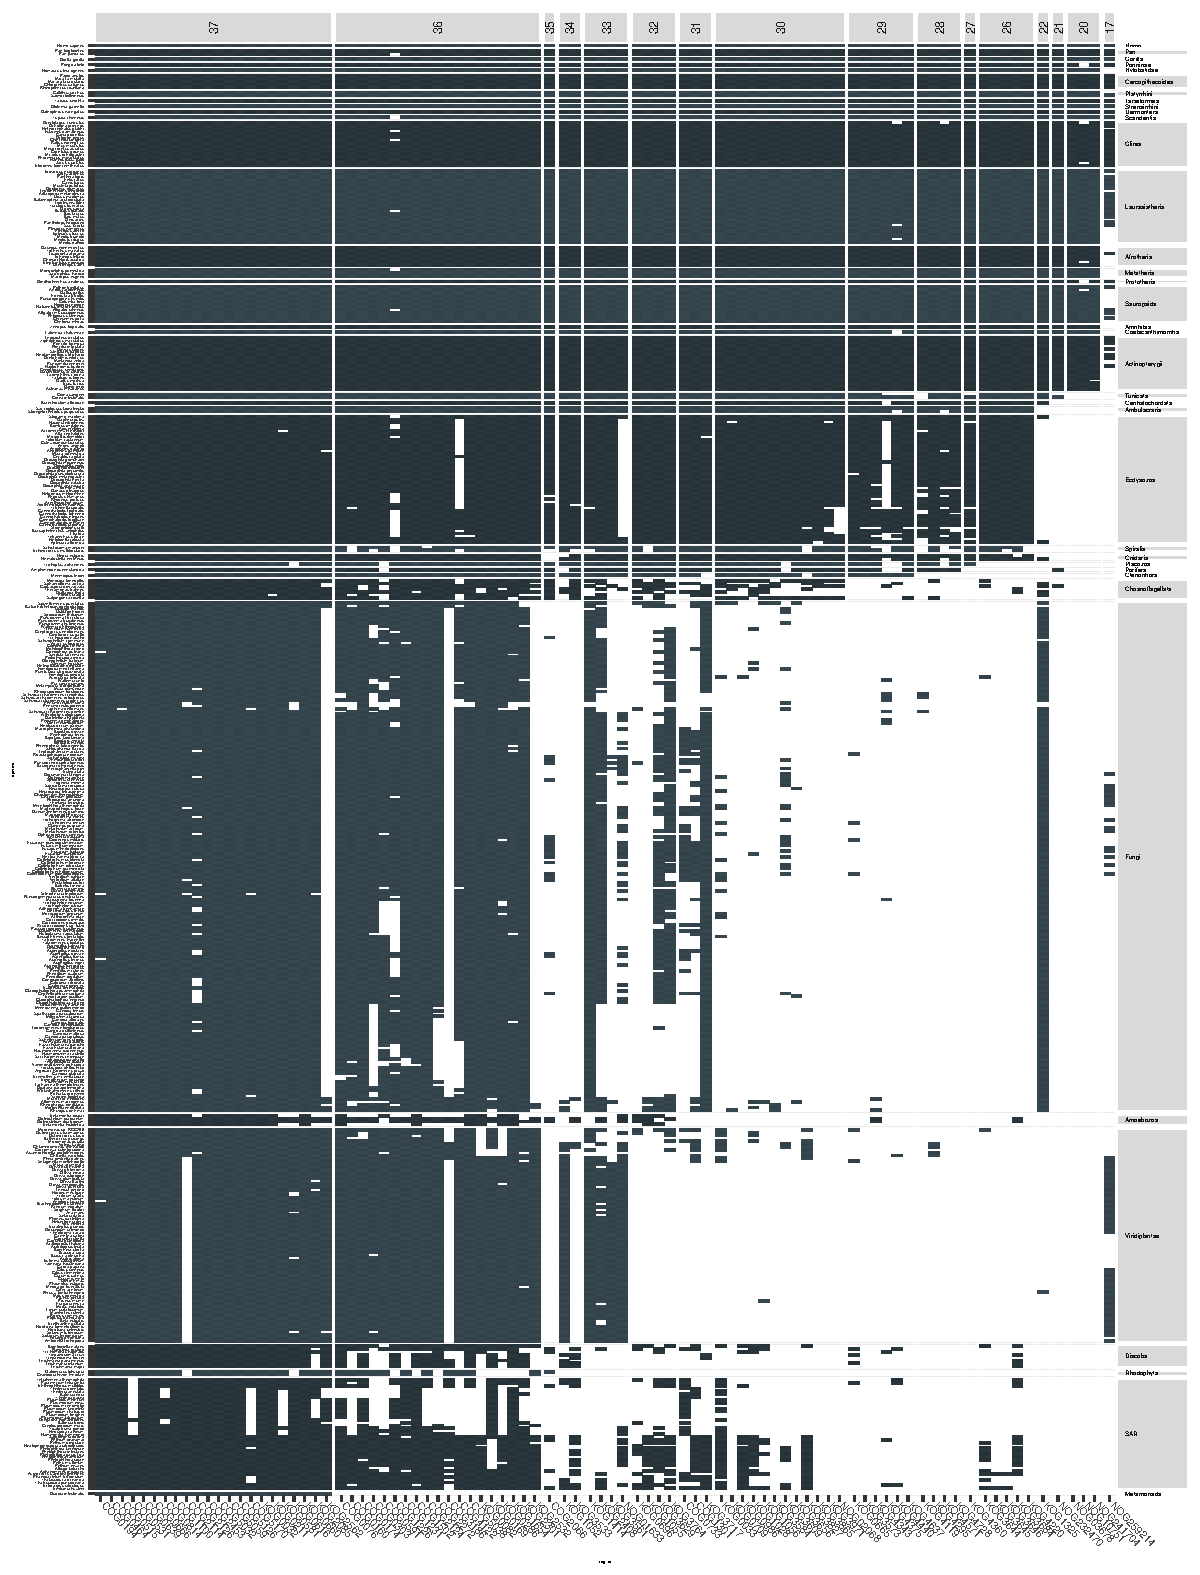
\includegraphics{figs/analysis.geneplast.unnamed-chunk-7-1} 

}

\caption{Presence of orthologous groups in species. The horizontal axis is grouped by COGs rooted at some specific LCA. The vertical axis is grouped by species' clades. A checkerboard pattern is superimposed to aid visual examination.}\label{fig:unnamed-chunk-7}
\end{figure}
